\section{Modo Protegido}

\subsection{Niveles de protección}

Intel soporta 4 niveles de protección diferentes, siendo 0 el mas alto y 3 el mas bajo. Por esa razón los bits de protección tienen 2 bits.

\begin{figure}[h!]
  \centering
    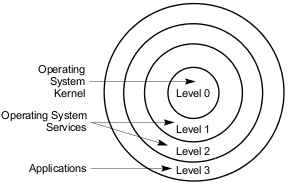
\includegraphics[width=0.3\textwidth]{images/protection_rings}
  \caption{Protection Rings}
\end{figure}

Si el $max(CPL, RPL) > DPL$ (recordemos que un nivel de protección mayor numérico se corresponde a un menor nivel de privilegio) al querer acceder o hacer un salto a un segmento, la \texttt{Unidad de Protección} verifica que no tenemos privilegios suficientes y el procesador nos da un General Protection Fault (\#GP). Esto se puede ver en la siguiente figura:

\begin{figure}[H]
  \centering
    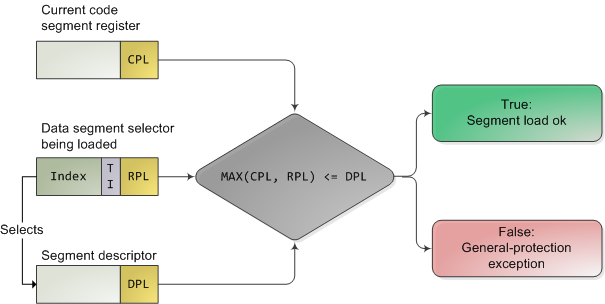
\includegraphics[width=0.6\textwidth]{images/protection}
  \caption{Protection Diagram}
\end{figure}

\subsection{Memory Management Unit}

Un procesador Intel, para gestionar lo que son los accesos a memoria, utiliza una \texttt{MMU} (Memory Management Unit). La misma esta compuesta por la Unidad de Segmentación y la Unidad de Paginación. La siguiente figura ilustra la idea general:

\begin{figure}[H]
  \centering
    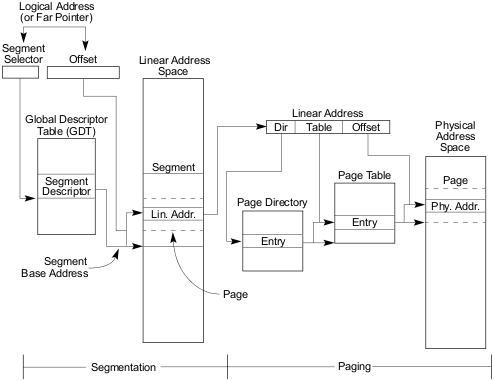
\includegraphics[width=0.4\textwidth]{images/memory_management}
  \caption{Segmentation \& Paging}
\end{figure}

\subsubsection{Unidad de Segmentación}

La unidad de segmentación se ocupa de pasar desde las \textit{direcciones lógicas} a \textit{direcciones lineales}. Su comportamiento está determinado por los \textit{registros de segmentación} (todos los que terminan en s), los mismos deben cargarse con el offset en la GDT del descriptor de segmento, permitiéndole a la CPU identificar el segmento adecuado dado un address lineal, la unidad de protección se ocupará de verificar que el \texttt{DPL} es compatible con el \texttt{CPL} y el \texttt{RPL}.

Por lo tanto, al entrar a modo protegido, lo primero que hacemos es inicializar los diferentes selectores de segmento. Los mismos tienen el siguiente formato:

\begin{figure}[h!]
  \centering
    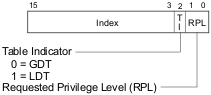
\includegraphics[scale=0.8]{images/segment_selector}
  \caption{Segment Selector}
\end{figure}

El index corresponde al descriptor de segmento en la \texttt{GDT}. Nosotros no utilizaremos la LDT, por lo que el bit TI estará siempre en 0. Ademas el \texttt{RPL} (Requested Protection Level) estará siempre en nivel 0 (superuser) o en 3 (usuario).

En modo protegido, los selectores de segmento tienen 16 bits. Los 13 bits mas significativos contienen el índice dentro de la tabla de descriptores. El bit 2 especifica si la operación utiliza la \texttt{GDT} o la \texttt{LDT}. Finalmente, los 2 bits menos significativos definen el nivel de privilegio solicitado.

\subsubsection{Unidad de Paginación}

Para activar la paginación, en primer lugar debemos inicializar el directorio de paginas y cargar el registro \reg{cr3} con la dirección del mismo. Como los directorios de paginas están alineados a 4 kB, los primeros 12 bits del \reg{cr3} no son necesarios para identificar el directorio, por lo que son utilizados por atributos del procesador. En nuestro caso no utilizamos estos atributos, por lo que son todos 0. La siguiente tabla muestra el formato del \reg{cr3}.

\begin{figure}[H]
  \centering
    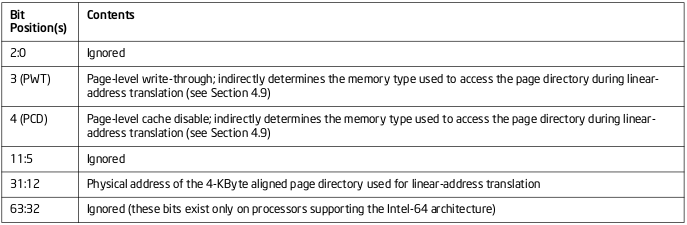
\includegraphics[width=0.8\textwidth]{images/cr3}
  \caption{CR3 Format}
\end{figure}

Luego activamos la paginación con el ultimo bit del registro \reg{cr0}. Una vez activada, la dirección lineal comienza a pasar luego por la unidad de paginación. La unidad de paginación se encarga de ir desde la dirección lineal a la dirección física en memoria. En caso de que la dirección lineal no este paginada, el procesador tiene una Page Fault Exception (\#PF).

Para facilitar el manejo y armado de estructuras de paginación, creamos varias funciones en C. Como sabemos, cada directorio de paginas tiene 1024 entradas de descriptores de 4 bytes. Lo mismo sucede con los directorios de paginas, que también tienen 1024 entradas con descriptores de 4 bytes. El procesador, al buscar estas estructuras en memoria RAM, requiere que las mismas estén alineadas a 4 kB, dado que es el tamaño de pagina que carga en memoria cache. A continuación, una breve explicación de qué hacen las funciones exportadas al usuario (cabe destacar, hay numerosos comentarios en el código explicando las particularidades):

\begin{itemize}
\item \fun{int mmap(uint virtualAddress, uint physicalAddress, uint directoryBase, uchar readWrite, uchar supervisorUser)}: mapea la página donde se encuentra el address virtual a la página donde se encuentra el address físico, indicando permisos de escritura o de usuario según se indique por parámetro.

\item \fun{int munmap(uint directoryBase, uint virtualAddress)}: desmapea la página donde se encuentra el address virtual.

\item \fun{int remap(uint directoryBase, uint virtualAddress, uint physicalAddress)}: Remapea la página donde se encuentra el address virtual a la página donde se encuentra el address físico.

\item \fun{int isMapped(uint directoryBase, uint virtualAddress)}: Devuelve true si, y solo si, la página donde se encuentra el address virtual está presente, es decir, si el address virtual es accesible.

\item \fun{int mmu\_move\_codepage(uint directoryBase, uint codeBaseSrc, uint codeBaseDst)}: Copia 1 página de memoria (4 KB) desde el primer address virtual hacia le segundo address virtual. Es importante tener en cuenta los page boundaries, porque el código va a generar un page fault si no hay suficiente espacio.
\end{itemize}

No es necesario inicializar ninguna estructura particular fuera de estar a nivel kernel para utilizar estas funciones. Es importante marcar que por el esquema de memoria que armamos, estas funciones pueden actuar sobre cualquier directorio de tablas de página, aun sin ser el propio. Es decir, no es necesario cambiar el \reg{cr3} para manipular la paginación de una tarea, sino que basta con tener acceso de escritura al directorio y tablas de páginas correspondientes.

\subsection{Interrupt Descriptor Table}

Una interrupción es una señal que le indica a la CPU que debe interrumpir la ejecución actual de instrucciones. El rol de la \texttt{IDT} (Interrupt Descriptor Table) es contener los diferentes descriptores de interrupción y asociar las diferentes interrupciones a sus respectivas rutinas de atención de interrupción. Existen tres fuentes de interrupciones:

\begin{enumerate}
\item Hardware: donde la interrupción proviene de un dispositivo conectado directamente al procesador, como por ejemplo el timer, o el teclado.
\item Software: en las que el mismo software llama al sistema, esto se utiliza para poder hacer cambios de nivel de privilegio, permitiendo al kernel exponer un conjunto de servicios común a todos los programas corriendo en la máquina.
\item Internas: que pertenecen estrictamente al procesador y ocurren, por ejemplo, cuando hay errores graves. La excepción de división por 0 es uno de estos casos.
\end{enumerate}

A su vez, la \texttt{IDT} puede contener tres tipos de descriptores:

\begin{enumerate}
\item Interrupt Gate
\item Trap Gate
\item Task Gate
\end{enumerate}

Para construir la IDT, armamos primero en C la estructura \texttt{idt\_entry} con sus respectivos atributos y luego construimos un array de 256 posiciones del mismo (la máxima cantidad soportada por el PIC). En este trabajo practico solo utilizaremos descriptores de interrupción y de tarea.

\begin{figure}[h!]
  \centering
    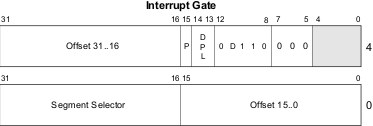
\includegraphics[width=0.5\textwidth]{images/idt_desc}
  \caption{IDT Descriptor}
\end{figure}

Modificamos la macro de la cátedra para poder cargar la IDT con diferentes atributos. Luego inicializamos las diferentes posiciones que utilizamos con sus respectivos selectores de segmento y atributos, tomando también la referencia a las respectivas rutinas de atención.

Hay que tener mucho cuidado al settear los atributos. Caso contrario, al cambiar de segmento podemos tener un General Protection Fault (\#GP). Algunos atributos son:

\begin{enumerate}
\item P: Present flag. 1 if present.
\item DPL: Descriptor Protection Level. Nivel de privilegios del descriptor.
\item D: Size of gate. 1 = 32 bits; 0 = 16 bits.
\end{enumerate}

Un procesador Intel reserva por default las primeras 31 posiciones de la \texttt{IDT} para las diferentes excepciones del procesador. Actualmente, el procesador solo utiliza las primeras 21. Inicializamos estas excepciones del procesador a una rutina que guarda el estado del procesador al suceder la primera interrupción y en caso de ser necesario desaloja la tarea actual. También inicializamos otros descriptores para atender otras interrupciones como la del reloj y la del teclado.

Una vez cargada la IDT, se debe remapear el PIC (Programmable Interrupt Controler) para referir a las nuevas interrupciones que agreguemos. Esto se hace con las rutinas de la cátedra \texttt{resetear\_pic} y luego \texttt{habilitar\_pic}.

\subsection{Otras Interrupciones}

Para inicializar otras interrupciones, tenemos que agregar los diferentes descriptores a la IDT, que apuntan a su correspondiente rutina de atención y además tienen los atributos correctos. Recordemos que las rutinas de atención de la interrupción deben ser transparentes a lo que el procesador estaba ejecutando en el momento, por lo que se deben guardar todos los registros utilizados y luego restaurarlos al finalizar la rutina de atención. Además, las interrupciones en general llevan a un escalamiento de privilegios, por lo que los privilegios también deben ser restaurados.

A su vez, la rutina de atención de la interrupción debe indicarle al pic que la interrupción esta siendo atendida, para que otras interrupciones puedan suceder. Esto se hace con la rutina de la cátedra \fun{fin\_intr\_pic1}.

\subsubsection{Reloj}

Esta es una interrupción interna, que sucede con cada \texttt{tick} del reloj del procesador. La rutina de atención de esta interrupción se encarga de mostrar la animación de un cursor rotando en la esquina inferior derecha de la pantalla, por medio de la función \fun{screen\_actualizar\_reloj\_global}. Luego haremos que llame al Scheduler y haga el switch de tareas.

\subsubsection{Teclado}
Utilizaremos la rutina de atención del teclado para habilitar las diferentes teclas disponibles a los jugadores. Cuando programábamos esto, notamos que es necesario tomar la tecla presionada desde el controlador del teclado, caso contrario el teclado no vuelve a solicitar una interrupción.

\subsubsection{Software}
Asignamos a la interrupción \addr{0x46} (70) una rutina que atiende un servicio del sistema.

\subsection{Entorno multi-tarea}

Para inicializar el entorno multi tearea, es importante definir entradas de \texttt{TSS} (Task State Segment) en la GDT. Cada una de estas entradas tienen bits distribuidos como la imágen de abajo, y declaran para una tarea cualquiera dónde se encontrará su Task State Segment correspondiente.

\begin{figure}[H]
  \centering
    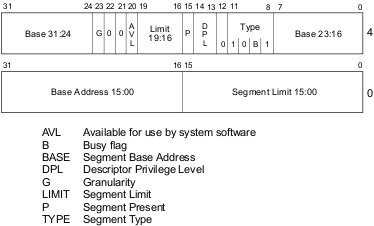
\includegraphics[width=0.5\textwidth]{images/tss_descriptor}
  \caption{TSS Descriptor}
\end{figure}

El Task State Segment es una estructura determinada por Intel, con fines de proveer un mecanismo automatizado que cumple con el propósito de guardar todo el contexto de ejecución del programa, facilitando la lógica necesaria para armar un entorno multi-tareas: el procesador se encarga automáticamente de todo el guardado y la carga de registros, ayudándonos a mantener una lógica más simple y correcta a nivel código. La siguiente figura describe la distribución de bits en un TSS:

\begin{figure}[H]
  \centering
    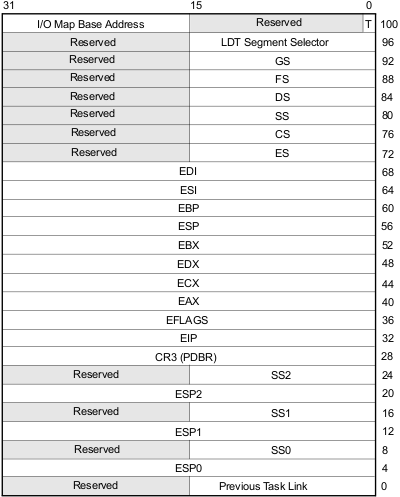
\includegraphics[width=0.3\textwidth]{images/tss}
  \caption{Task State Segment}
\end{figure}

Estas estructuras deben ser inicializadas con cuidado: es muy importante que cada tarea tenga una pila de nivel 0 bien configurada, una pila de nivel 3, los segmentos de datos y código bien definidos (¡es importante destacar que en el caso de las tareas a nivel usuario hay que declarar los permisos adecuados!), el \reg{eip}, y el \reg{iomap} deshabilitado. Además las \reg{EFLAGS} deben estar puestas en 0x202, ya que sino no tendremos interrupciones habilitadas.

La última pieza del mecanismo es el registro \reg{TR} (Task Register), que contiene todo el tiempo el offset del selector de segmento de TSS correspondiente a la tarea actual. El mismo tiene una parte oculta que cachea el descriptor de segmento correspondiente al selector. Las instrucciones \texttt{LTR} y \texttt{STR} nos permiten cargar y guardar el Task Register, asumiendo que tenemos \texttt{CPL} 0.

\begin{figure}[H]
  \centering
    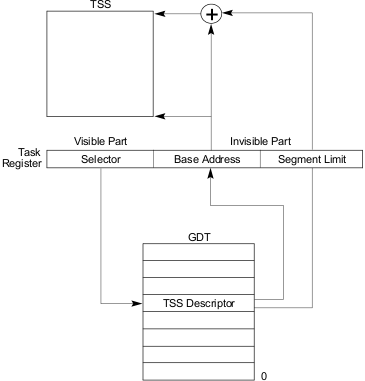
\includegraphics[width=0.3\textwidth]{images/task_register}
  \caption{Segmentation \& Paging}
\end{figure}

Para llamar a una tarea, se lleva a cabo un \texttt{jmp far} con su respectivo selector de segmento (el offset no se utiliza). El procesador se ocupa de guardar el contexto de la tarea actual en la TSS correspondiente al \reg{TR}, y de cargar el nuevo contexto de ejecución.

En nuestro kernel, definimos un total de 18 tareas: la inicial, la idle, y las 16 tareas de piratas correspondientes a los jugadores. La tarea inicial tiene como propósito guardar el contexto antes de realizar el primer task switch, mientras que la tarea idle funciona como un placeholder cuando no tenemos una tarea de usuario para ejecutar. Por lo tanto, la forma de inicializar multi tasking es cargando el registro \reg{TR} con la tarea inicial, haciendo luego un task switch a la tarea Idle. Cabe destacar que es importante tener habilitadas las interrupciones antes de saltar a la tarea Idle, ya que sino no podremos ni lanzar piratas, ni ejecutar código de los mismos.